\section{Programm}\label{Programm}
Um die Methoden der Threads in einer Realen Situation zu nutzen, habe ich mich entschlossen ein Programm, welches stark von Threads profitieren kann, zu programmieren.  

Ich habe mich für ein Programm eintscheiden, mit dem man ein Bild mit vielen weiteren Bildern rekrieren kann. Es wird demnach ein Mosaik aus Bildern erstellt.

\begin{figure}[h]
    \centering
    \subfloat[\centering Input]{
        
\includegraphics[height=5cm]{images/Source_100x100.pdf}
    }
    \subfloat[\centering Output]{
        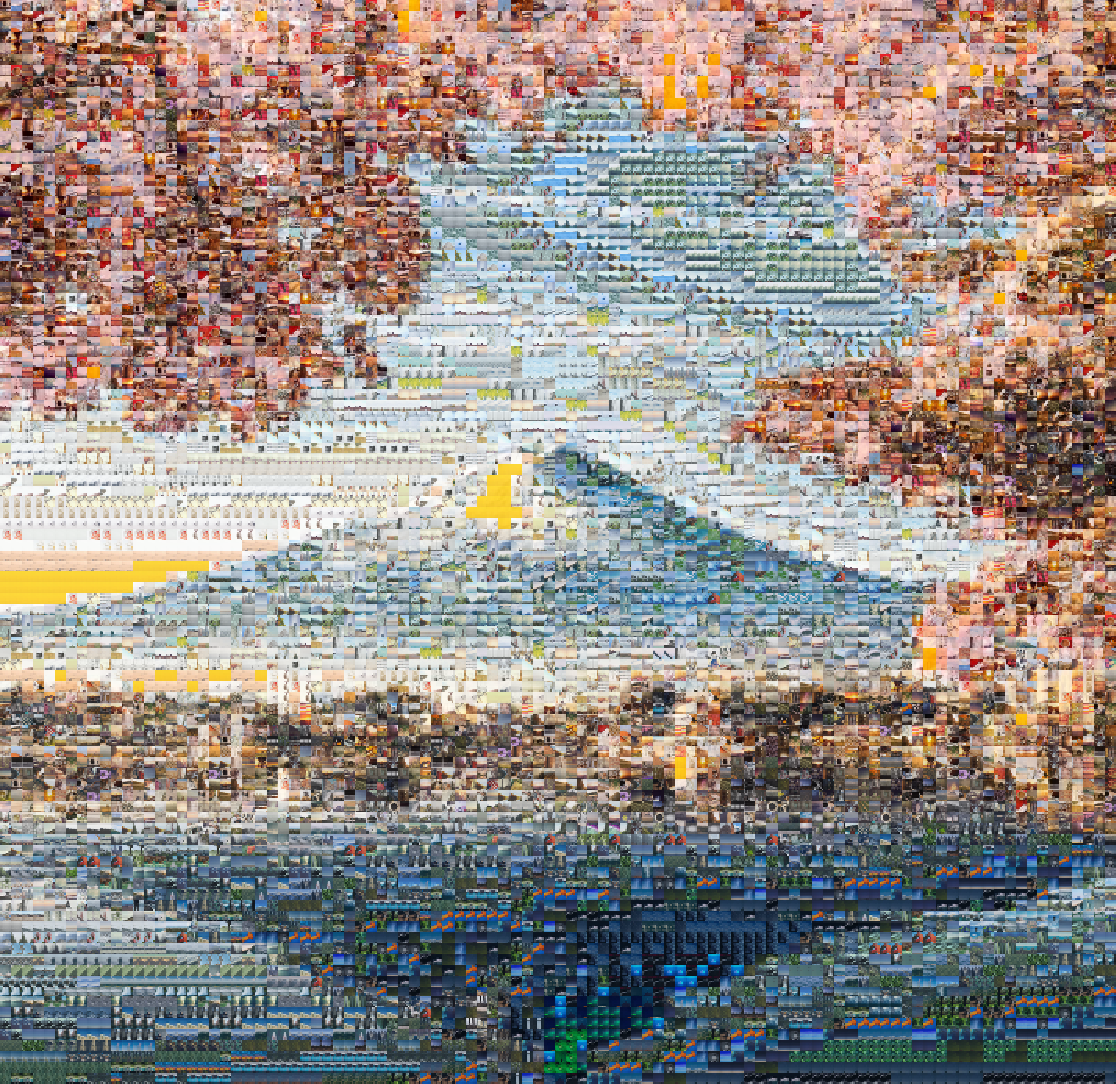
\includegraphics[height=5cm]{images/Render_100x100.pdf}
    }
    \caption[Programm Funktion]{Funktionsweise des Programmes}
\end{figure}

Die anwendung von Threads kommt in dem Programm in vielen Stellen vor. Im folgen werde ich mich auf den Algorythmus der Bild analyse und verarbeitung beziehen. Andere aspekte, wie die implementation des Testmodus und andere Features, die in der App vorhanden sind, werden kurz im Anhang erwähnt.